\documentclass[12px]{article}

\title{Lezione 5 Fisica Generale I}
\date{2024-10-09}
\author{Federico De Sisti}

\usepackage{amsmath}
\usepackage{amsthm}
\usepackage{mdframed}
\usepackage{amssymb}
\usepackage{nicematrix}
\usepackage{amsfonts}
\usepackage{tcolorbox}
\tcbuselibrary{theorems}
\usepackage{xcolor}
\usepackage{cancel}

\newtheoremstyle{break}
  {1px}{1px}%
  {\itshape}{}%
  {\bfseries}{}%
  {\newline}{}%
\theoremstyle{break}
\newtheorem{theo}{Teorema}
\theoremstyle{break}
\newtheorem{lemma}{Lemma}
\theoremstyle{break}
\newtheorem{defin}{Definizione}
\theoremstyle{break}
\newtheorem{propo}{Proposizione}
\theoremstyle{break}
\newtheorem*{dimo}{Dimostrazione}
\theoremstyle{break}
\newtheorem*{es}{Esempio}

\newenvironment{dimo}
  {\begin{dimostrazione}}
  {\hfill\square\end{dimostrazione}}

\newenvironment{teo}
{\begin{mdframed}[linecolor=red, backgroundcolor=red!10]\begin{theo}}
  {\end{theo}\end{mdframed}}

\newenvironment{nome}
{\begin{mdframed}[linecolor=green, backgroundcolor=green!10]\begin{nomen}}
  {\end{nomen}\end{mdframed}}

\newenvironment{prop}
{\begin{mdframed}[linecolor=red, backgroundcolor=red!10]\begin{propo}}
  {\end{propo}\end{mdframed}}

\newenvironment{defi}
{\begin{mdframed}[linecolor=orange, backgroundcolor=orange!10]\begin{defin}}
  {\end{defin}\end{mdframed}}

\newenvironment{lemm}
{\begin{mdframed}[linecolor=red, backgroundcolor=red!10]\begin{lemma}}
  {\end{lemma}\end{mdframed}}

\newcommand{\icol}[1]{% inline column vector
  \left(\begin{smallmatrix}#1\end{smallmatrix}\right)%
}

\newcommand{\irow}[1]{% inline row vector
  \begin{smallmatrix}(#1)\end{smallmatrix}%
}

\newcommand{\matrice}[1]{% inline column vector
  \begin{pmatrix}#1\end{pmatrix}%
}

\newcommand{\C}{\mathbb{C}}
\newcommand{\K}{\mathbb{K}}
\newcommand{\R}{\mathbb{R}}


\begin{document}
	\maketitle
	\newpage
	\section{Chissà}\\
	$v(t_1) = v_2 \ \ \x(t_1) = x_2$\\
	$v(t) = v_1 + a(t-t_1)$\\
	$x(t) = x_2 + v_1(t-t_2) = \frac a 2 \left[ \left(t-t_1)^2 + (t_2-t_1)^2\right] $\\
		Se $t_1 = t_2 = 0$\\
		$x(t) = x_2 + v_1(t-t_1) + \frac a 2 (t-t_1)^2$\\
		$t_1 = t_2 = 0$\\
		$x(t) = x_0 + v_0t + \frac a 2 t^2$\\
		Dimostrare che questa equazione del moto fa qualcosa di poco chiaro (per esercizio)\\
		\[
			x(t_2) = x_2 = x_0 + v_0t_2 + \frac 1 2 a t^2_2
		.\] 
		\[
		v(t_1) = v_1 = v_0 + at_1
		.\] \begin{tikzpicture}
    % Draw axes
    \draw[->] (-2,0) -- (2,0) node[right] {$x$};
    \draw[->] (0,-2) -- (0,2) node[above] {$y$};

    % Draw unit circle
    \draw (0,0) circle(1);

    % Draw angle theta
    \draw[thick] (0,0) -- (30:1) node[midway, below right] {$\theta (t)$} node[midway,above] {$\overrightarrow{r}(t)$};
    \draw[->, thick] (0.5,0) arc[start angle=0, end angle=30, radius=0.5];

    % Label point on the circle
\end{tikzpicture}\\
\begin{center}
	
\begin{cases}
	x(t) = r\cos\theta(t)\\
	y(t) = r\sin\theta(t)
\end{cases}\\
\begin{cases}
	v_x(t) = -r\sin\theta(t)v(t)\\
	v_y(t) = r\cos\theta(t)v(t)
\end{cases}\\
\begin{cases}
	a_x(t) = -r\cos\theta(t)[\theta(t)]^2 - r\sin\theta(t)\theta(t)\\
	a_y(t) = -r\sin\theta(t)[\theta(t)]^2 + r\cos\theta(t)\theta(t)\\
\end{cases}
\end{center}
\[
	\theta(t)'' = \frac{d^2\theta}{dt^2} = \diff {\omega(t)} t = \alpha(t)
.\] 
\[
	v(t) = \sqrt{v_x(t)^2 + v_y(t)^2} = r\theta(t) = r\omega (t)
.\] 
\[
	a(t) = \sqrt{a_x^2(t) + a^2_y(t)} = \sqrt{r^2\theta'(t) + r^2\theta'(t)
\] 
\[
	=\sqrt {r^2 \omega^2(t) + r^2 \alpha^2(t)} = \sqrt{a_c^2 + a_t^2}
.\] 
\[
	\theta'(t) = \diff {\theta(t)} t
.\] 
Nel caso del moto circolare uniforme\\
$\omega = cost = \diff {\theta(t)} t \ \ \ \ \ \theta_0 = \theta(0)$
\[
\theta(t) = \theta_0 + \omega t = \varphi + \omega t
.\] 
Dove $ \varphi$ è la condizione iniziale dell'angolo\\
\[
\begin{cases}
	x(t) = r\cos(\omega t + \varphi) = r\cos(\theta(t))\\
	y(t) = r\sin(\omega t + \varphi) = r\sin(\theta(t))
\end{cases}
.\] 
\subsection{Moto circolare uniformemente accellerato}
$\alpha = cost$\\
 \[
\diff \omega t \alpha \Rightarrow \omega (t) = \omega_0 + \alpha t
.\] 
\[
\diff \theta t = \omega(t) \Rightarrow \theta (t) = \theta_0 + \omega t + \frac 1 2 \alpha t^2 
.\] 
\[
	\theta_0 = \omega_0 = 0 - \theta(t) - \frac 1 2 \alpha t^2
.\] 
\[
	a(t) = \sqrt{r^2\theta'(t)^4 + r^2\theta''(t)^2} = \sqrt{r^2\omega^4(t) + r^2\alpha^ 2} 
.\] 
\[
= \sqrt{r^2\alpha^4t^4 + r^2\alpha^2} = r\alpha\sqrt{\alpha^2t^2 + 1}
.\] 
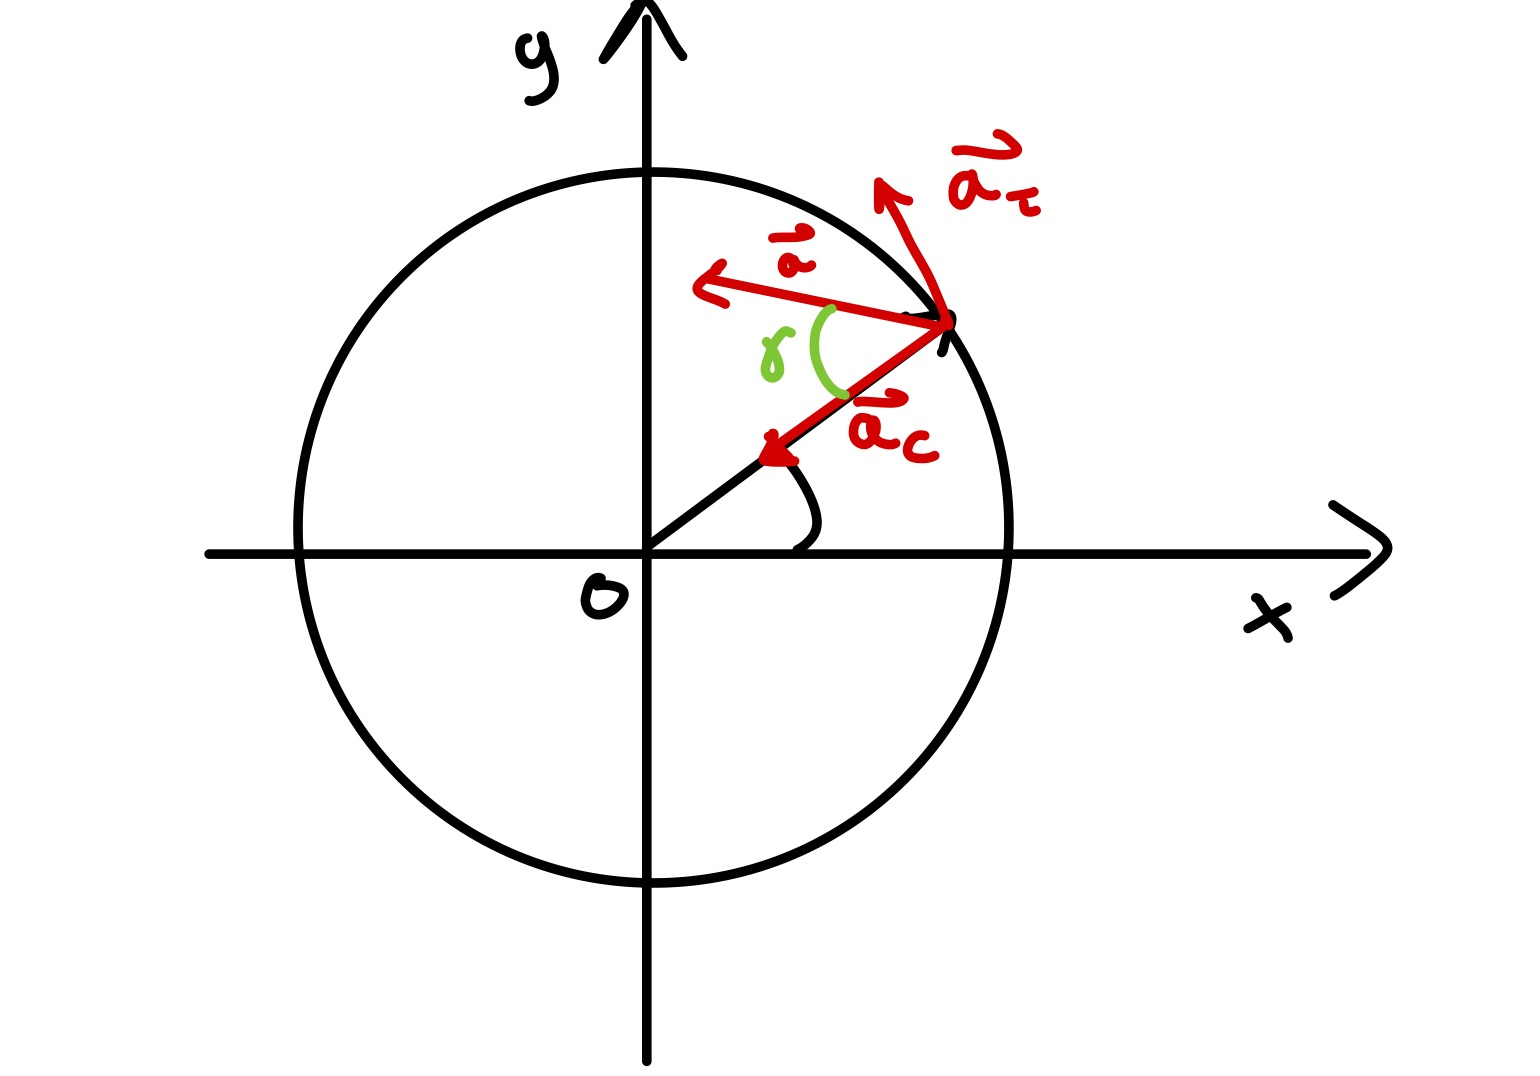
\includegraphics[scale=0.2]{cerchio_1}\\
\begin{cases}
	a_t = a\sin\gamma\\
	a_c = a\cos\gamma
\end{cases}\\
\[\gamma = \arctan\frac{a_t}{a_c} \ \ \gamma = \arctan \frac 1 {\alpha t^2}\]
\textbf{Esercizio:}\\
Ho un orologio in cui le lancette segnano le 3:00\\
Dopo quanto tempo le lancette formeranno un anoglo di $\pi/2 $ tra di loro?\\
\textbf{Svolgimento}\\
\[T_ore = 12 h \ \ \ T_minuti = 1h \ \ \omega_{ore} = \frac {2\pi}{T_{ore}} \ \ \ \ \omega_{minuti} = \frac {2\pi}{T_{minuti}}\]\\
$\theta(t) = \theta_0 + \omega t$\\
$\theta_{ore}(t) = \omega_{ore}t$\\
$\theta_{minuti}(t) = - \frac \pi 2 \omega_{minuti}t$\\
Dobbiamo trovare il più piccolo $t^*$ tale che\\
$\theta_{ore}(t^*)-\theta_{minuti}(t^*) = \pm \frac \pi 2 + 2k\pi$ con  $k\in \mathbb Z$\\
 \[
	 \frac {2\pi} {12 h} t^* - \frac {2\pi}{1 h} t^* + \frac \pi 2 = \pm \frac \pi 2 + 2 k\pi
.\] 
Proviamo prima con il $+$ e poicon il  $-$ \\
$n=0$
 \[
	 t^*_+ = \frac {12}{11} h
.\] 
ora, con il $-$\\
 \[
	 t^*_- = \frac {6}{11} h < t^*_+
.\] 
%TODO PARTE CHE MANCA
$a = 2 m/s$\\
 $v$ dopo $5s$\\
 $v_m$ in $[0,5]s$
  \[
 v(t) = at
 .\] 
 \[
 v(t=5s) = 2 m/s^2 \cdot 5 s = 10m/s
 .\] 
 \[
	 2) v_m = \frac{x(t=5s) - x(t=0s)}{\Delta t}
 .\]
 \[
x(t_0) = x(0) + v(0)t + \frac 12 at^2
 .\] 
 \[
 \Delta x = x(t) - x(0) = v(0)t + \frac 12 at^2
 .\] 
 \[
	 \overline v = \frac{v(0) + v(t^*)} 2 = \frac {10} 2  m/s = 5m/s
 
 .\] 
 \textbf{Esempio:}\\
 Una macchina va, ad una velocità di $v = 100 km/h$\\
  $a = -5 m/s^2$\\
  $1)\Delta x = x(t) - x(0) = ?$\\
   $2)$ quanti ci mette?\\
   \textbf{Svolgimento}\\
   1)
   \[
	   x(t) - x(0) = \Delta x = \frac{v(t)^2- v(0)^2}{2a}
   .\] 
   Dove $t^*$ è il tempo in cui la macchina si ferma
   \[
	   x(t^*) - x(0) = \frac{v(t^*) - v(0)^2}{2a} = - \frac{v(0)^2}{2a} = 77 m
   .\] 
   2)
   \[
   v(t) = v(0) + at
   .\] 
   \[
   v(t^*) = 0 = v(0)+ at^*
   .\] 
   \[
	   t^* = 5.5 s
   .\] 
Con il tempo di reazione?\\
reazione = $0.5s$\\
$x(t) = x_0 + vt$\\
$x(t_{frenata}) - x_0 = vt_{reazione}$ \\
Problema inverso, ho lo stesso tempo di reazione, se voglio fermarmi dopo 100 metri, qual'è la velocità massima che posso tenere?\\
\[
	x(t_{frenata}) - x_0 = vt_{reazione}
.\] 
\[
	v(0)t_{reazione} = \frac{v(0)^2}{2a}\leq\Delta x_{max}
.\] 
\[
	v_{max}t_{reazione} - \frac{v_{max}^2}{2a} - \Delta x_{max} = 0
.\] 
\[
	-2av_{max}t_{max} + v_{max}^2 + 2a\Delta x_{max}=0
.\] 
\[
	v_{max} = at_{reazione}\pm\sqrt{a^2t_{max}^2-2a\Delta x_max}
.\] 

\end{document}
